\documentclass[twoside]{book}

% Packages required by doxygen
\usepackage{calc}
\usepackage{doxygen}
\usepackage{graphicx}
\usepackage[utf8]{inputenc}
\usepackage{makeidx}
\usepackage{multicol}
\usepackage{multirow}
\usepackage{textcomp}
\usepackage[table]{xcolor}

% Font selection
\usepackage[T1]{fontenc}
\usepackage{mathptmx}
\usepackage[scaled=.90]{helvet}
\usepackage{courier}
\usepackage{amssymb}
\usepackage{sectsty}
\renewcommand{\familydefault}{\sfdefault}
\allsectionsfont{%
  \fontseries{bc}\selectfont%
  \color{darkgray}%
}
\renewcommand{\DoxyLabelFont}{%
  \fontseries{bc}\selectfont%
  \color{darkgray}%
}

% Page & text layout
\usepackage{geometry}
\geometry{%
  a4paper,%
  top=2.5cm,%
  bottom=2.5cm,%
  left=2.5cm,%
  right=2.5cm%
}
\tolerance=750
\hfuzz=15pt
\hbadness=750
\setlength{\emergencystretch}{15pt}
\setlength{\parindent}{0cm}
\setlength{\parskip}{0.2cm}
\makeatletter
\renewcommand{\paragraph}{%
  \@startsection{paragraph}{4}{0ex}{-1.0ex}{1.0ex}{%
    \normalfont\normalsize\bfseries\SS@parafont%
  }%
}
\renewcommand{\subparagraph}{%
  \@startsection{subparagraph}{5}{0ex}{-1.0ex}{1.0ex}{%
    \normalfont\normalsize\bfseries\SS@subparafont%
  }%
}
\makeatother

% Headers & footers
\usepackage{fancyhdr}
\pagestyle{fancyplain}
\fancyhead[LE]{\fancyplain{}{\bfseries\thepage}}
\fancyhead[CE]{\fancyplain{}{}}
\fancyhead[RE]{\fancyplain{}{\bfseries\leftmark}}
\fancyhead[LO]{\fancyplain{}{\bfseries\rightmark}}
\fancyhead[CO]{\fancyplain{}{}}
\fancyhead[RO]{\fancyplain{}{\bfseries\thepage}}
\fancyfoot[LE]{\fancyplain{}{}}
\fancyfoot[CE]{\fancyplain{}{}}
\fancyfoot[RE]{\fancyplain{}{\bfseries\scriptsize Generated on Tue Jul 1 2014 23\-:45\-:09 for Remote Sensing by Doxygen }}
\fancyfoot[LO]{\fancyplain{}{\bfseries\scriptsize Generated on Tue Jul 1 2014 23\-:45\-:09 for Remote Sensing by Doxygen }}
\fancyfoot[CO]{\fancyplain{}{}}
\fancyfoot[RO]{\fancyplain{}{}}
\renewcommand{\footrulewidth}{0.4pt}
\renewcommand{\chaptermark}[1]{%
  \markboth{#1}{}%
}
\renewcommand{\sectionmark}[1]{%
  \markright{\thesection\ #1}%
}

% Indices & bibliography
\usepackage{natbib}
\usepackage[titles]{tocloft}
\setcounter{tocdepth}{3}
\setcounter{secnumdepth}{5}
\makeindex

% Hyperlinks (required, but should be loaded last)
\usepackage{ifpdf}
\ifpdf
  \usepackage[pdftex,pagebackref=true]{hyperref}
\else
  \usepackage[ps2pdf,pagebackref=true]{hyperref}
\fi
\hypersetup{%
  colorlinks=true,%
  linkcolor=blue,%
  citecolor=blue,%
  unicode%
}

% Custom commands
\newcommand{\clearemptydoublepage}{%
  \newpage{\pagestyle{empty}\cleardoublepage}%
}


%===== C O N T E N T S =====

\begin{document}

% Titlepage & ToC
\hypersetup{pageanchor=false}
\pagenumbering{roman}
\begin{titlepage}
\vspace*{7cm}
\begin{center}%
{\Large Remote Sensing }\\
\vspace*{1cm}
{\large Generated by Doxygen 1.8.6}\\
\vspace*{0.5cm}
{\small Tue Jul 1 2014 23:45:09}\\
\end{center}
\end{titlepage}
\clearemptydoublepage
\tableofcontents
\clearemptydoublepage
\pagenumbering{arabic}
\hypersetup{pageanchor=true}

%--- Begin generated contents ---
\chapter{Remote Sensing}
\label{index}\hypertarget{index}{}\hypertarget{index_information}{}\section{Information}\label{index_information}
This program collects data from the hardware sensors, then converts it to a readable unit (Celsius, etc), and uploads it to a server.

We only need one python file to accomplish this, and that file is \hyperlink{sensing_8py}{sensing.\-py}. This single file depends on the pypcduino library however, and that code is also included.

The appropriate documentation is included within.\hypertarget{index_authors}{}\section{Authors}\label{index_authors}
Made by\-:
\begin{DoxyItemize}
\item Justin Mc\-Bride
\item Austin Cerny
\item Reed Anderson
\item Aaron Holt
\end{DoxyItemize}\hypertarget{index_hardwareinfo}{}\section{Hardware Information}\label{index_hardwareinfo}
This python script runs on several pc\-Duino v2 boards located in different places.

Each unit has various sensors attached to it, and for whatever sensor they have, the appropriate data is uploaded.\hypertarget{index_serverinfo}{}\section{Server Information}\label{index_serverinfo}
The server is a Ubuntu instance on Amazon's E\-C2 infrastructure. The server runs Mongo\-D\-B and listens for input through a R\-E\-S\-T A\-P\-I generated by a Dream\-Factory instance. The server also utilizes Angular.\-J\-S to create a graphical frontend for the information.\hypertarget{index_requirements}{}\section{Requirements to Run}\label{index_requirements}
This code requires the external library 'requests'.\hypertarget{index_testing}{}\section{Testing}\label{index_testing}
Unit testing is enabled through the python unittest module.

To run the tests, simply use the terminal command

\$ python \hyperlink{test__sensing_8py}{test\-\_\-sensing.\-py}\hypertarget{index_static}{}\section{Static Analysis}\label{index_static}
This code utilizes the pylint module to perform static analysis on the code. Simply run

\$ pylint \hyperlink{sensing_8py}{sensing.\-py}

to generate a report. A generated pylintrc directive file is included with the code to supress the following error messages\-:

{\itshape missing-\/docstring} -\/ Doxygen uses a different format than docstrings for documentation.

{\itshape invalid-\/name} -\/ We're not following Py\-Lint's Style guide.

{\itshape mixed-\/indentation} -\/ Using spaces in Doxygen documentation confuses Py\-Lint

{\itshape anomalous-\/backslash-\/in-\/string} -\/ Doxygen uses backslashes in the documentation markdown.

{\itshape trailing-\/whitespace} -\/ Also used in Doxygen formatting.\hypertarget{index_documents}{}\section{Documentation}\label{index_documents}
The documentation for this code was created with the use of Doxygen. Because Doxygen does not natively (at least completely) support Python, the use of Doxypy from \href{http://code.foosel.org/doxypy}{\tt http\-://code.\-foosel.\-org/doxypy} is used as an input filter. 
\chapter{Namespace Index}
\section{Namespace List}
Here is a list of all namespaces with brief descriptions\-:\begin{DoxyCompactList}
\item\contentsline{section}{\hyperlink{namespacepypcduino}{pypcduino} }{\pageref{namespacepypcduino}}{}
\item\contentsline{section}{\hyperlink{namespacepypcduino_1_1adc}{pypcduino.\-adc} }{\pageref{namespacepypcduino_1_1adc}}{}
\item\contentsline{section}{\hyperlink{namespacepypcduino_1_1exceptions}{pypcduino.\-exceptions} }{\pageref{namespacepypcduino_1_1exceptions}}{}
\item\contentsline{section}{\hyperlink{namespacepypcduino_1_1gpio}{pypcduino.\-gpio} }{\pageref{namespacepypcduino_1_1gpio}}{}
\item\contentsline{section}{\hyperlink{namespacepypcduino_1_1pinmap}{pypcduino.\-pinmap} }{\pageref{namespacepypcduino_1_1pinmap}}{}
\item\contentsline{section}{\hyperlink{namespacesensing}{sensing} }{\pageref{namespacesensing}}{}
\end{DoxyCompactList}

\chapter{Hierarchical Index}
\section{Class Hierarchy}
This inheritance list is sorted roughly, but not completely, alphabetically\-:\begin{DoxyCompactList}
\item Exception\begin{DoxyCompactList}
\item \contentsline{section}{sensing.\-Sensor\-Name\-Exception}{\pageref{classsensing_1_1_sensor_name_exception}}{}
\item \contentsline{section}{sensing.\-Sensor\-Pin\-Exception}{\pageref{classsensing_1_1_sensor_pin_exception}}{}
\end{DoxyCompactList}
\item object\begin{DoxyCompactList}
\item \contentsline{section}{pypcduino.\-pinmap.\-Pin\-Map}{\pageref{classpypcduino_1_1pinmap_1_1_pin_map}}{}
\item \contentsline{section}{sensing.\-Light\-Sensor}{\pageref{classsensing_1_1_light_sensor}}{}
\item \contentsline{section}{sensing.\-Temperature\-Sensor}{\pageref{classsensing_1_1_temperature_sensor}}{}
\end{DoxyCompactList}
\item Test\-Case\begin{DoxyCompactList}
\item \contentsline{section}{test\-\_\-sensing.\-Test\-Sensing}{\pageref{classtest__sensing_1_1_test_sensing}}{}
\end{DoxyCompactList}
\item Value\-Error\begin{DoxyCompactList}
\item \contentsline{section}{pypcduino.\-pinmap.\-Invalid\-Channel\-Exception}{\pageref{classpypcduino_1_1pinmap_1_1_invalid_channel_exception}}{}
\end{DoxyCompactList}
\end{DoxyCompactList}

\chapter{Class Index}
\section{Class List}
Here are the classes, structs, unions and interfaces with brief descriptions\-:\begin{DoxyCompactList}
\item\contentsline{section}{\hyperlink{classpypcduino_1_1pinmap_1_1_invalid_channel_exception}{pypcduino.\-pinmap.\-Invalid\-Channel\-Exception} \\*The channel sent was invalid }{\pageref{classpypcduino_1_1pinmap_1_1_invalid_channel_exception}}{}
\item\contentsline{section}{\hyperlink{classsensing_1_1_light_sensor}{sensing.\-Light\-Sensor} \\*The class for a light sensor Contains all the functions to get data about the light }{\pageref{classsensing_1_1_light_sensor}}{}
\item\contentsline{section}{\hyperlink{classsensing_1_1_no_history_exception}{sensing.\-No\-History\-Exception} \\*An exception that would be raised when a sensor's history list is empty }{\pageref{classsensing_1_1_no_history_exception}}{}
\item\contentsline{section}{\hyperlink{classpypcduino_1_1pinmap_1_1_pin_map}{pypcduino.\-pinmap.\-Pin\-Map} }{\pageref{classpypcduino_1_1pinmap_1_1_pin_map}}{}
\item\contentsline{section}{\hyperlink{classsensing_1_1_pin_read_out_of_range_exception}{sensing.\-Pin\-Read\-Out\-Of\-Range\-Exception} \\*An exception that should occur when a pin reads out of range (0-\/4096) }{\pageref{classsensing_1_1_pin_read_out_of_range_exception}}{}
\item\contentsline{section}{\hyperlink{classsensing_1_1_sensor_name_exception}{sensing.\-Sensor\-Name\-Exception} \\*An exception to get thrown when a sensor was set up with an invalid name }{\pageref{classsensing_1_1_sensor_name_exception}}{}
\item\contentsline{section}{\hyperlink{classsensing_1_1_sensor_pin_exception}{sensing.\-Sensor\-Pin\-Exception} \\*An exception to get thrown when a sensor was set up with an invalid pin location }{\pageref{classsensing_1_1_sensor_pin_exception}}{}
\item\contentsline{section}{\hyperlink{classsensing_1_1_temperature_sensor}{sensing.\-Temperature\-Sensor} \\*The class for a Temperature Sensor It has the functions to get the temperature and parse it }{\pageref{classsensing_1_1_temperature_sensor}}{}
\item\contentsline{section}{\hyperlink{classtest__sensing_1_1_test_sensing}{test\-\_\-sensing.\-Test\-Sensing} }{\pageref{classtest__sensing_1_1_test_sensing}}{}
\end{DoxyCompactList}

\chapter{File Index}
\section{File List}
Here is a list of all files with brief descriptions\-:\begin{DoxyCompactList}
\item\contentsline{section}{/home/justin/\-C\-S\-C\-I\-Project/pcduino/\hyperlink{sensing_8py}{sensing.\-py} }{\pageref{sensing_8py}}{}
\item\contentsline{section}{/home/justin/\-C\-S\-C\-I\-Project/pcduino/\hyperlink{test__sensing_8py}{test\-\_\-sensing.\-py} }{\pageref{test__sensing_8py}}{}
\item\contentsline{section}{/home/justin/\-C\-S\-C\-I\-Project/pcduino/pypcduino/\hyperlink{____init_____8py}{\-\_\-\-\_\-init\-\_\-\-\_\-.\-py} }{\pageref{____init_____8py}}{}
\item\contentsline{section}{/home/justin/\-C\-S\-C\-I\-Project/pcduino/pypcduino/\hyperlink{adc_8py}{adc.\-py} }{\pageref{adc_8py}}{}
\item\contentsline{section}{/home/justin/\-C\-S\-C\-I\-Project/pcduino/pypcduino/\hyperlink{exceptions_8py}{exceptions.\-py} }{\pageref{exceptions_8py}}{}
\item\contentsline{section}{/home/justin/\-C\-S\-C\-I\-Project/pcduino/pypcduino/\hyperlink{gpio_8py}{gpio.\-py} }{\pageref{gpio_8py}}{}
\item\contentsline{section}{/home/justin/\-C\-S\-C\-I\-Project/pcduino/pypcduino/\hyperlink{pinmap_8py}{pinmap.\-py} }{\pageref{pinmap_8py}}{}
\end{DoxyCompactList}

\chapter{Namespace Documentation}
\hypertarget{namespacepypcduino}{\section{pypcduino Namespace Reference}
\label{namespacepypcduino}\index{pypcduino@{pypcduino}}
}
\subsection*{Namespaces}
\begin{DoxyCompactItemize}
\item 
\hyperlink{namespacepypcduino_1_1adc}{adc}
\item 
\hyperlink{namespacepypcduino_1_1exceptions}{exceptions}
\item 
\hyperlink{namespacepypcduino_1_1gpio}{gpio}
\item 
\hyperlink{namespacepypcduino_1_1pinmap}{pinmap}
\end{DoxyCompactItemize}

\hypertarget{namespacepypcduino_1_1adc}{\section{pypcduino.\-adc Namespace Reference}
\label{namespacepypcduino_1_1adc}\index{pypcduino.\-adc@{pypcduino.\-adc}}
}
\subsection*{Functions}
\begin{DoxyCompactItemize}
\item 
def \hyperlink{namespacepypcduino_1_1adc_a3ef1a506a5cb668cf5b418c804facbcd}{analog\-\_\-read}
\begin{DoxyCompactList}\small\item\em Return the integer value of an adc pin. \end{DoxyCompactList}\end{DoxyCompactItemize}
\subsection*{Variables}
\begin{DoxyCompactItemize}
\item 
tuple \hyperlink{namespacepypcduino_1_1adc_a766105e33e35d9fa020e87c19e6ddf07}{pins} = Pin\-Map('/proc', 'adc', 6)
\end{DoxyCompactItemize}


\subsection{Function Documentation}
\hypertarget{namespacepypcduino_1_1adc_a3ef1a506a5cb668cf5b418c804facbcd}{\index{pypcduino\-::adc@{pypcduino\-::adc}!analog\-\_\-read@{analog\-\_\-read}}
\index{analog\-\_\-read@{analog\-\_\-read}!pypcduino::adc@{pypcduino\-::adc}}
\subsubsection[{analog\-\_\-read}]{\setlength{\rightskip}{0pt plus 5cm}def pypcduino.\-adc.\-analog\-\_\-read (
\begin{DoxyParamCaption}
\item[{}]{channel}
\end{DoxyParamCaption}
)}}\label{namespacepypcduino_1_1adc_a3ef1a506a5cb668cf5b418c804facbcd}


Return the integer value of an adc pin. 

adc0 and adc1 have 6 bit resolution. adc2 through adc5 have 12 bit resolution. 

\subsection{Variable Documentation}
\hypertarget{namespacepypcduino_1_1adc_a766105e33e35d9fa020e87c19e6ddf07}{\index{pypcduino\-::adc@{pypcduino\-::adc}!pins@{pins}}
\index{pins@{pins}!pypcduino::adc@{pypcduino\-::adc}}
\subsubsection[{pins}]{\setlength{\rightskip}{0pt plus 5cm}tuple pypcduino.\-adc.\-pins = Pin\-Map('/proc', 'adc', 6)}}\label{namespacepypcduino_1_1adc_a766105e33e35d9fa020e87c19e6ddf07}

\hypertarget{namespacepypcduino_1_1exceptions}{\section{pypcduino.\-exceptions Namespace Reference}
\label{namespacepypcduino_1_1exceptions}\index{pypcduino.\-exceptions@{pypcduino.\-exceptions}}
}

\hypertarget{namespacepypcduino_1_1gpio}{\section{pypcduino.\-gpio Namespace Reference}
\label{namespacepypcduino_1_1gpio}\index{pypcduino.\-gpio@{pypcduino.\-gpio}}
}
\subsection*{Functions}
\begin{DoxyCompactItemize}
\item 
def \hyperlink{namespacepypcduino_1_1gpio_aba7c287e8da39dc2e5f7951ebe7819a4}{digital\-\_\-write}
\begin{DoxyCompactList}\small\item\em Write to a G\-P\-I\-O channel. \end{DoxyCompactList}\item 
def \hyperlink{namespacepypcduino_1_1gpio_aa324a331fb50643f94e222b8eef38fe8}{digital\-\_\-read}
\begin{DoxyCompactList}\small\item\em Read from a G\-P\-I\-O channel. \end{DoxyCompactList}\item 
def \hyperlink{namespacepypcduino_1_1gpio_af0917a2382b59c8825b60df9cc4d6830}{pin\-\_\-mode}
\begin{DoxyCompactList}\small\item\em Set Mode of a G\-P\-I\-O channel. \end{DoxyCompactList}\end{DoxyCompactItemize}
\subsection*{Variables}
\begin{DoxyCompactItemize}
\item 
list \hyperlink{namespacepypcduino_1_1gpio_a8a55cdc8c6b775ffa9ba8aa68cfd8d93}{\-\_\-\-\_\-all\-\_\-\-\_\-}
\item 
int \hyperlink{namespacepypcduino_1_1gpio_a017380b78afe9853e0cc3ca009c47ec3}{H\-I\-G\-H} = 1
\item 
int \hyperlink{namespacepypcduino_1_1gpio_a7794534b6aba1a94e2ed468ec8fbed98}{L\-O\-W} = 0
\item 
int \hyperlink{namespacepypcduino_1_1gpio_afabe8a2ce86d5db92f8e5994e5c24252}{I\-N\-P\-U\-T} = 0
\item 
int \hyperlink{namespacepypcduino_1_1gpio_a810c8642dc31f28d747c4c845e8a4a80}{O\-U\-T\-P\-U\-T} = 1
\item 
tuple \hyperlink{namespacepypcduino_1_1gpio_acf2dcb151997749e99dbf65c08073e08}{gpio\-\_\-pins}
\item 
tuple \hyperlink{namespacepypcduino_1_1gpio_a3e40fb727c6bb0d0f1bcf69478a9a1c0}{gpio\-\_\-mode\-\_\-pins}
\end{DoxyCompactItemize}


\subsection{Function Documentation}
\hypertarget{namespacepypcduino_1_1gpio_aa324a331fb50643f94e222b8eef38fe8}{\index{pypcduino\-::gpio@{pypcduino\-::gpio}!digital\-\_\-read@{digital\-\_\-read}}
\index{digital\-\_\-read@{digital\-\_\-read}!pypcduino::gpio@{pypcduino\-::gpio}}
\subsubsection[{digital\-\_\-read}]{\setlength{\rightskip}{0pt plus 5cm}def pypcduino.\-gpio.\-digital\-\_\-read (
\begin{DoxyParamCaption}
\item[{}]{channel}
\end{DoxyParamCaption}
)}}\label{namespacepypcduino_1_1gpio_aa324a331fb50643f94e222b8eef38fe8}


Read from a G\-P\-I\-O channel. 

\hypertarget{namespacepypcduino_1_1gpio_aba7c287e8da39dc2e5f7951ebe7819a4}{\index{pypcduino\-::gpio@{pypcduino\-::gpio}!digital\-\_\-write@{digital\-\_\-write}}
\index{digital\-\_\-write@{digital\-\_\-write}!pypcduino::gpio@{pypcduino\-::gpio}}
\subsubsection[{digital\-\_\-write}]{\setlength{\rightskip}{0pt plus 5cm}def pypcduino.\-gpio.\-digital\-\_\-write (
\begin{DoxyParamCaption}
\item[{}]{channel, }
\item[{}]{value}
\end{DoxyParamCaption}
)}}\label{namespacepypcduino_1_1gpio_aba7c287e8da39dc2e5f7951ebe7819a4}


Write to a G\-P\-I\-O channel. 

\hypertarget{namespacepypcduino_1_1gpio_af0917a2382b59c8825b60df9cc4d6830}{\index{pypcduino\-::gpio@{pypcduino\-::gpio}!pin\-\_\-mode@{pin\-\_\-mode}}
\index{pin\-\_\-mode@{pin\-\_\-mode}!pypcduino::gpio@{pypcduino\-::gpio}}
\subsubsection[{pin\-\_\-mode}]{\setlength{\rightskip}{0pt plus 5cm}def pypcduino.\-gpio.\-pin\-\_\-mode (
\begin{DoxyParamCaption}
\item[{}]{channel, }
\item[{}]{mode}
\end{DoxyParamCaption}
)}}\label{namespacepypcduino_1_1gpio_af0917a2382b59c8825b60df9cc4d6830}


Set Mode of a G\-P\-I\-O channel. 



\subsection{Variable Documentation}
\hypertarget{namespacepypcduino_1_1gpio_a8a55cdc8c6b775ffa9ba8aa68cfd8d93}{\index{pypcduino\-::gpio@{pypcduino\-::gpio}!\-\_\-\-\_\-all\-\_\-\-\_\-@{\-\_\-\-\_\-all\-\_\-\-\_\-}}
\index{\-\_\-\-\_\-all\-\_\-\-\_\-@{\-\_\-\-\_\-all\-\_\-\-\_\-}!pypcduino::gpio@{pypcduino\-::gpio}}
\subsubsection[{\-\_\-\-\_\-all\-\_\-\-\_\-}]{\setlength{\rightskip}{0pt plus 5cm}list pypcduino.\-gpio.\-\_\-\-\_\-all\-\_\-\-\_\-}}\label{namespacepypcduino_1_1gpio_a8a55cdc8c6b775ffa9ba8aa68cfd8d93}
{\bfseries Initial value\-:}
\begin{DoxyCode}
1 = [\textcolor{stringliteral}{'HIGH'}, \textcolor{stringliteral}{'LOW'}, \textcolor{stringliteral}{'INPUT'}, \textcolor{stringliteral}{'OUTPUT'},\textcolor{stringliteral}{'digital\_write'}, \textcolor{stringliteral}{'digital\_read'},
2            \textcolor{stringliteral}{"pin\_mode"}]
\end{DoxyCode}
\hypertarget{namespacepypcduino_1_1gpio_a3e40fb727c6bb0d0f1bcf69478a9a1c0}{\index{pypcduino\-::gpio@{pypcduino\-::gpio}!gpio\-\_\-mode\-\_\-pins@{gpio\-\_\-mode\-\_\-pins}}
\index{gpio\-\_\-mode\-\_\-pins@{gpio\-\_\-mode\-\_\-pins}!pypcduino::gpio@{pypcduino\-::gpio}}
\subsubsection[{gpio\-\_\-mode\-\_\-pins}]{\setlength{\rightskip}{0pt plus 5cm}tuple pypcduino.\-gpio.\-gpio\-\_\-mode\-\_\-pins}}\label{namespacepypcduino_1_1gpio_a3e40fb727c6bb0d0f1bcf69478a9a1c0}
{\bfseries Initial value\-:}
\begin{DoxyCode}
1 = PinMap(
2     \textcolor{stringliteral}{'/sys/devices/virtual/misc/gpio/mode/'},
3     \textcolor{stringliteral}{'gpio'},
4     20
5 )
\end{DoxyCode}
\hypertarget{namespacepypcduino_1_1gpio_acf2dcb151997749e99dbf65c08073e08}{\index{pypcduino\-::gpio@{pypcduino\-::gpio}!gpio\-\_\-pins@{gpio\-\_\-pins}}
\index{gpio\-\_\-pins@{gpio\-\_\-pins}!pypcduino::gpio@{pypcduino\-::gpio}}
\subsubsection[{gpio\-\_\-pins}]{\setlength{\rightskip}{0pt plus 5cm}tuple pypcduino.\-gpio.\-gpio\-\_\-pins}}\label{namespacepypcduino_1_1gpio_acf2dcb151997749e99dbf65c08073e08}
{\bfseries Initial value\-:}
\begin{DoxyCode}
1 = PinMap(
2     \textcolor{stringliteral}{'/sys/devices/virtual/misc/gpio/pin'},
3     \textcolor{stringliteral}{'gpio'},
4     20
5 )
\end{DoxyCode}
\hypertarget{namespacepypcduino_1_1gpio_a017380b78afe9853e0cc3ca009c47ec3}{\index{pypcduino\-::gpio@{pypcduino\-::gpio}!H\-I\-G\-H@{H\-I\-G\-H}}
\index{H\-I\-G\-H@{H\-I\-G\-H}!pypcduino::gpio@{pypcduino\-::gpio}}
\subsubsection[{H\-I\-G\-H}]{\setlength{\rightskip}{0pt plus 5cm}int pypcduino.\-gpio.\-H\-I\-G\-H = 1}}\label{namespacepypcduino_1_1gpio_a017380b78afe9853e0cc3ca009c47ec3}
\hypertarget{namespacepypcduino_1_1gpio_afabe8a2ce86d5db92f8e5994e5c24252}{\index{pypcduino\-::gpio@{pypcduino\-::gpio}!I\-N\-P\-U\-T@{I\-N\-P\-U\-T}}
\index{I\-N\-P\-U\-T@{I\-N\-P\-U\-T}!pypcduino::gpio@{pypcduino\-::gpio}}
\subsubsection[{I\-N\-P\-U\-T}]{\setlength{\rightskip}{0pt plus 5cm}int pypcduino.\-gpio.\-I\-N\-P\-U\-T = 0}}\label{namespacepypcduino_1_1gpio_afabe8a2ce86d5db92f8e5994e5c24252}
\hypertarget{namespacepypcduino_1_1gpio_a7794534b6aba1a94e2ed468ec8fbed98}{\index{pypcduino\-::gpio@{pypcduino\-::gpio}!L\-O\-W@{L\-O\-W}}
\index{L\-O\-W@{L\-O\-W}!pypcduino::gpio@{pypcduino\-::gpio}}
\subsubsection[{L\-O\-W}]{\setlength{\rightskip}{0pt plus 5cm}int pypcduino.\-gpio.\-L\-O\-W = 0}}\label{namespacepypcduino_1_1gpio_a7794534b6aba1a94e2ed468ec8fbed98}
\hypertarget{namespacepypcduino_1_1gpio_a810c8642dc31f28d747c4c845e8a4a80}{\index{pypcduino\-::gpio@{pypcduino\-::gpio}!O\-U\-T\-P\-U\-T@{O\-U\-T\-P\-U\-T}}
\index{O\-U\-T\-P\-U\-T@{O\-U\-T\-P\-U\-T}!pypcduino::gpio@{pypcduino\-::gpio}}
\subsubsection[{O\-U\-T\-P\-U\-T}]{\setlength{\rightskip}{0pt plus 5cm}int pypcduino.\-gpio.\-O\-U\-T\-P\-U\-T = 1}}\label{namespacepypcduino_1_1gpio_a810c8642dc31f28d747c4c845e8a4a80}

\hypertarget{namespacepypcduino_1_1pinmap}{\section{pypcduino.\-pinmap Namespace Reference}
\label{namespacepypcduino_1_1pinmap}\index{pypcduino.\-pinmap@{pypcduino.\-pinmap}}
}
\subsection*{Classes}
\begin{DoxyCompactItemize}
\item 
class \hyperlink{classpypcduino_1_1pinmap_1_1_invalid_channel_exception}{Invalid\-Channel\-Exception}
\begin{DoxyCompactList}\small\item\em The channel sent was invalid. \end{DoxyCompactList}\item 
class \hyperlink{classpypcduino_1_1pinmap_1_1_pin_map}{Pin\-Map}
\end{DoxyCompactItemize}

\hypertarget{namespacesensing}{\section{sensing Namespace Reference}
\label{namespacesensing}\index{sensing@{sensing}}
}
\subsection*{Functions}
\begin{DoxyCompactItemize}
\item 
def \hyperlink{namespacesensing_a110922c2a80aabf038d162595e137cc4}{delay}
\begin{DoxyCompactList}\small\item\em Put the program to sleep for a specified number of seconds. \end{DoxyCompactList}\item 
def \hyperlink{namespacesensing_afc4f85f529614a384ee1d04cd5ff80f3}{loop}
\begin{DoxyCompactList}\small\item\em This is where the program will spend the majority of its time, looping through indefinitely. \end{DoxyCompactList}\item 
def \hyperlink{namespacesensing_aeae2450fef0f1a9244c1ddc6d96ef4c2}{send\-Data}
\begin{DoxyCompactList}\small\item\em Here we actually ship off the information to the server. \end{DoxyCompactList}\item 
def \hyperlink{namespacesensing_a75479ff0f15da4027d590f94160bb43f}{update\-Pin\-Readings}
\begin{DoxyCompactList}\small\item\em This function will read the values reported by the hardware, and then save that data to the appropriate sensor's variable. \end{DoxyCompactList}\item 
def \hyperlink{namespacesensing_a38d7f8a9b27bbcf471a89725a5e78493}{main}
\begin{DoxyCompactList}\small\item\em The entry point of the program. \end{DoxyCompactList}\end{DoxyCompactItemize}
\subsection*{Variables}
\begin{DoxyCompactItemize}
\item 
string \hyperlink{namespacesensing_a7d59d9b021482661d93cbf2120dfa030}{board\-Name} = 'Justin'
\begin{DoxyCompactList}\small\item\em A unique board I\-D to identify the individual board. \end{DoxyCompactList}\item 
int \hyperlink{namespacesensing_a299f408c66c5c07e7eb2392a01472dd7}{last\-Temperature} = 0
\begin{DoxyCompactList}\small\item\em A global variable to hold the last reading of the last temperature measured. \end{DoxyCompactList}\item 
int \hyperlink{namespacesensing_a763e931b762ad2fa2b4cdb6f815ffe00}{light\-Pin\-Reading} = 0
\begin{DoxyCompactList}\small\item\em A global variable to hold the last reading of the last light brightness measured. \end{DoxyCompactList}\item 
string \hyperlink{namespacesensing_a5de0b501e0135c4f0709266d12fa2814}{api\-U\-R\-I} = 'http\-://dsp-\/csci-\/project.\-cloud.\-dreamfactory.\-com/rest/mongodb/sensordata'
\begin{DoxyCompactList}\small\item\em This is the location of the R\-E\-S\-T A\-P\-I and it is where we will send our calls to. \end{DoxyCompactList}\item 
dictionary \hyperlink{namespacesensing_a10bdd4ea61df5e84854a462509e3c7d5}{headers} = \{'content-\/type' \-: 'application/json', 'X-\/Dream\-Factory-\/Application-\/Name' \-: 'Remote\-Sensing'\}
\begin{DoxyCompactList}\small\item\em These are the headers that we need to send with our R\-E\-S\-T A\-P\-I calls. \end{DoxyCompactList}\end{DoxyCompactItemize}


\subsection{Function Documentation}
\hypertarget{namespacesensing_a110922c2a80aabf038d162595e137cc4}{\index{sensing@{sensing}!delay@{delay}}
\index{delay@{delay}!sensing@{sensing}}
\subsubsection[{delay}]{\setlength{\rightskip}{0pt plus 5cm}def sensing.\-delay (
\begin{DoxyParamCaption}
\item[{}]{ms}
\end{DoxyParamCaption}
)}}\label{namespacesensing_a110922c2a80aabf038d162595e137cc4}


Put the program to sleep for a specified number of seconds. 

\hypertarget{namespacesensing_afc4f85f529614a384ee1d04cd5ff80f3}{\index{sensing@{sensing}!loop@{loop}}
\index{loop@{loop}!sensing@{sensing}}
\subsubsection[{loop}]{\setlength{\rightskip}{0pt plus 5cm}def sensing.\-loop (
\begin{DoxyParamCaption}
{}
\end{DoxyParamCaption}
)}}\label{namespacesensing_afc4f85f529614a384ee1d04cd5ff80f3}


This is where the program will spend the majority of its time, looping through indefinitely. 

\hypertarget{namespacesensing_a38d7f8a9b27bbcf471a89725a5e78493}{\index{sensing@{sensing}!main@{main}}
\index{main@{main}!sensing@{sensing}}
\subsubsection[{main}]{\setlength{\rightskip}{0pt plus 5cm}def sensing.\-main (
\begin{DoxyParamCaption}
{}
\end{DoxyParamCaption}
)}}\label{namespacesensing_a38d7f8a9b27bbcf471a89725a5e78493}


The entry point of the program. 

\hypertarget{namespacesensing_aeae2450fef0f1a9244c1ddc6d96ef4c2}{\index{sensing@{sensing}!send\-Data@{send\-Data}}
\index{send\-Data@{send\-Data}!sensing@{sensing}}
\subsubsection[{send\-Data}]{\setlength{\rightskip}{0pt plus 5cm}def sensing.\-send\-Data (
\begin{DoxyParamCaption}
{}
\end{DoxyParamCaption}
)}}\label{namespacesensing_aeae2450fef0f1a9244c1ddc6d96ef4c2}


Here we actually ship off the information to the server. 

\hypertarget{namespacesensing_a75479ff0f15da4027d590f94160bb43f}{\index{sensing@{sensing}!update\-Pin\-Readings@{update\-Pin\-Readings}}
\index{update\-Pin\-Readings@{update\-Pin\-Readings}!sensing@{sensing}}
\subsubsection[{update\-Pin\-Readings}]{\setlength{\rightskip}{0pt plus 5cm}def sensing.\-update\-Pin\-Readings (
\begin{DoxyParamCaption}
{}
\end{DoxyParamCaption}
)}}\label{namespacesensing_a75479ff0f15da4027d590f94160bb43f}


This function will read the values reported by the hardware, and then save that data to the appropriate sensor's variable. 



\subsection{Variable Documentation}
\hypertarget{namespacesensing_a5de0b501e0135c4f0709266d12fa2814}{\index{sensing@{sensing}!api\-U\-R\-I@{api\-U\-R\-I}}
\index{api\-U\-R\-I@{api\-U\-R\-I}!sensing@{sensing}}
\subsubsection[{api\-U\-R\-I}]{\setlength{\rightskip}{0pt plus 5cm}string sensing.\-api\-U\-R\-I = 'http\-://dsp-\/csci-\/project.\-cloud.\-dreamfactory.\-com/rest/mongodb/sensordata'}}\label{namespacesensing_a5de0b501e0135c4f0709266d12fa2814}


This is the location of the R\-E\-S\-T A\-P\-I and it is where we will send our calls to. 

\hypertarget{namespacesensing_a7d59d9b021482661d93cbf2120dfa030}{\index{sensing@{sensing}!board\-Name@{board\-Name}}
\index{board\-Name@{board\-Name}!sensing@{sensing}}
\subsubsection[{board\-Name}]{\setlength{\rightskip}{0pt plus 5cm}string sensing.\-board\-Name = 'Justin'}}\label{namespacesensing_a7d59d9b021482661d93cbf2120dfa030}


A unique board I\-D to identify the individual board. 

\hypertarget{namespacesensing_a10bdd4ea61df5e84854a462509e3c7d5}{\index{sensing@{sensing}!headers@{headers}}
\index{headers@{headers}!sensing@{sensing}}
\subsubsection[{headers}]{\setlength{\rightskip}{0pt plus 5cm}dictionary sensing.\-headers = \{'content-\/type' \-: 'application/json', 'X-\/Dream\-Factory-\/Application-\/Name' \-: 'Remote\-Sensing'\}}}\label{namespacesensing_a10bdd4ea61df5e84854a462509e3c7d5}


These are the headers that we need to send with our R\-E\-S\-T A\-P\-I calls. 

\hypertarget{namespacesensing_a299f408c66c5c07e7eb2392a01472dd7}{\index{sensing@{sensing}!last\-Temperature@{last\-Temperature}}
\index{last\-Temperature@{last\-Temperature}!sensing@{sensing}}
\subsubsection[{last\-Temperature}]{\setlength{\rightskip}{0pt plus 5cm}int sensing.\-last\-Temperature = 0}}\label{namespacesensing_a299f408c66c5c07e7eb2392a01472dd7}


A global variable to hold the last reading of the last temperature measured. 

\hypertarget{namespacesensing_a763e931b762ad2fa2b4cdb6f815ffe00}{\index{sensing@{sensing}!light\-Pin\-Reading@{light\-Pin\-Reading}}
\index{light\-Pin\-Reading@{light\-Pin\-Reading}!sensing@{sensing}}
\subsubsection[{light\-Pin\-Reading}]{\setlength{\rightskip}{0pt plus 5cm}int sensing.\-light\-Pin\-Reading = 0}}\label{namespacesensing_a763e931b762ad2fa2b4cdb6f815ffe00}


A global variable to hold the last reading of the last light brightness measured. 


\hypertarget{namespacetest__sensing}{\section{test\-\_\-sensing Namespace Reference}
\label{namespacetest__sensing}\index{test\-\_\-sensing@{test\-\_\-sensing}}
}
\subsection*{Classes}
\begin{DoxyCompactItemize}
\item 
class \hyperlink{classtest__sensing_1_1_test_sensing}{Test\-Sensing}
\end{DoxyCompactItemize}

\chapter{Class Documentation}
\hypertarget{classpypcduino_1_1pinmap_1_1_invalid_channel_exception}{\section{pypcduino.\-pinmap.\-Invalid\-Channel\-Exception Class Reference}
\label{classpypcduino_1_1pinmap_1_1_invalid_channel_exception}\index{pypcduino.\-pinmap.\-Invalid\-Channel\-Exception@{pypcduino.\-pinmap.\-Invalid\-Channel\-Exception}}
}


The channel sent was invalid.  


Inheritance diagram for pypcduino.\-pinmap.\-Invalid\-Channel\-Exception\-:\begin{figure}[H]
\begin{center}
\leavevmode
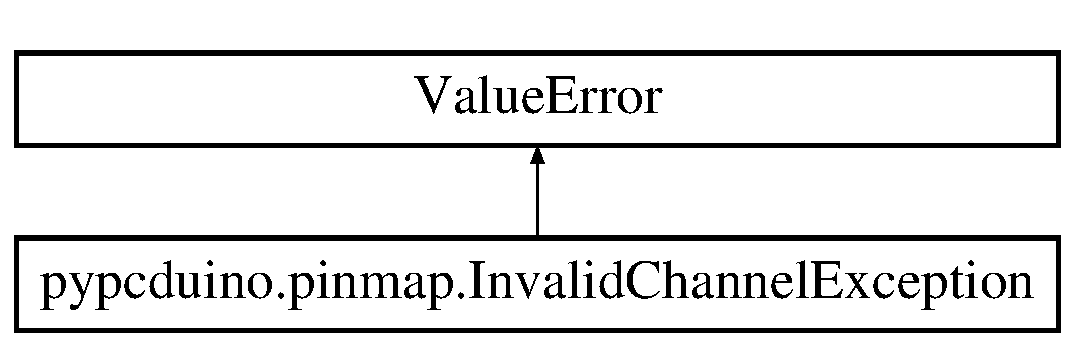
\includegraphics[height=2.000000cm]{classpypcduino_1_1pinmap_1_1_invalid_channel_exception}
\end{center}
\end{figure}
\subsection*{Public Member Functions}
\begin{DoxyCompactItemize}
\item 
def \hyperlink{classpypcduino_1_1pinmap_1_1_invalid_channel_exception_a2766b1ffd00966872fa613cb806b9ffa}{\-\_\-\-\_\-init\-\_\-\-\_\-}
\end{DoxyCompactItemize}


\subsection{Detailed Description}
The channel sent was invalid. 



\subsection{Constructor \& Destructor Documentation}
\hypertarget{classpypcduino_1_1pinmap_1_1_invalid_channel_exception_a2766b1ffd00966872fa613cb806b9ffa}{\index{pypcduino\-::pinmap\-::\-Invalid\-Channel\-Exception@{pypcduino\-::pinmap\-::\-Invalid\-Channel\-Exception}!\-\_\-\-\_\-init\-\_\-\-\_\-@{\-\_\-\-\_\-init\-\_\-\-\_\-}}
\index{\-\_\-\-\_\-init\-\_\-\-\_\-@{\-\_\-\-\_\-init\-\_\-\-\_\-}!pypcduino::pinmap::InvalidChannelException@{pypcduino\-::pinmap\-::\-Invalid\-Channel\-Exception}}
\subsubsection[{\-\_\-\-\_\-init\-\_\-\-\_\-}]{\setlength{\rightskip}{0pt plus 5cm}def pypcduino.\-pinmap.\-Invalid\-Channel\-Exception.\-\_\-\-\_\-init\-\_\-\-\_\- (
\begin{DoxyParamCaption}
\item[{}]{self, }
\item[{}]{pin}
\end{DoxyParamCaption}
)}}\label{classpypcduino_1_1pinmap_1_1_invalid_channel_exception_a2766b1ffd00966872fa613cb806b9ffa}


The documentation for this class was generated from the following file\-:\begin{DoxyCompactItemize}
\item 
/home/justin/\-C\-S\-C\-I\-Project/pcduino/pypcduino/\hyperlink{pinmap_8py}{pinmap.\-py}\end{DoxyCompactItemize}

\hypertarget{classsensing_1_1_light_sensor}{\section{sensing.\-Light\-Sensor Class Reference}
\label{classsensing_1_1_light_sensor}\index{sensing.\-Light\-Sensor@{sensing.\-Light\-Sensor}}
}


The class for a light sensor Contains all the functions to get data about the light.  


Inheritance diagram for sensing.\-Light\-Sensor\-:\begin{figure}[H]
\begin{center}
\leavevmode
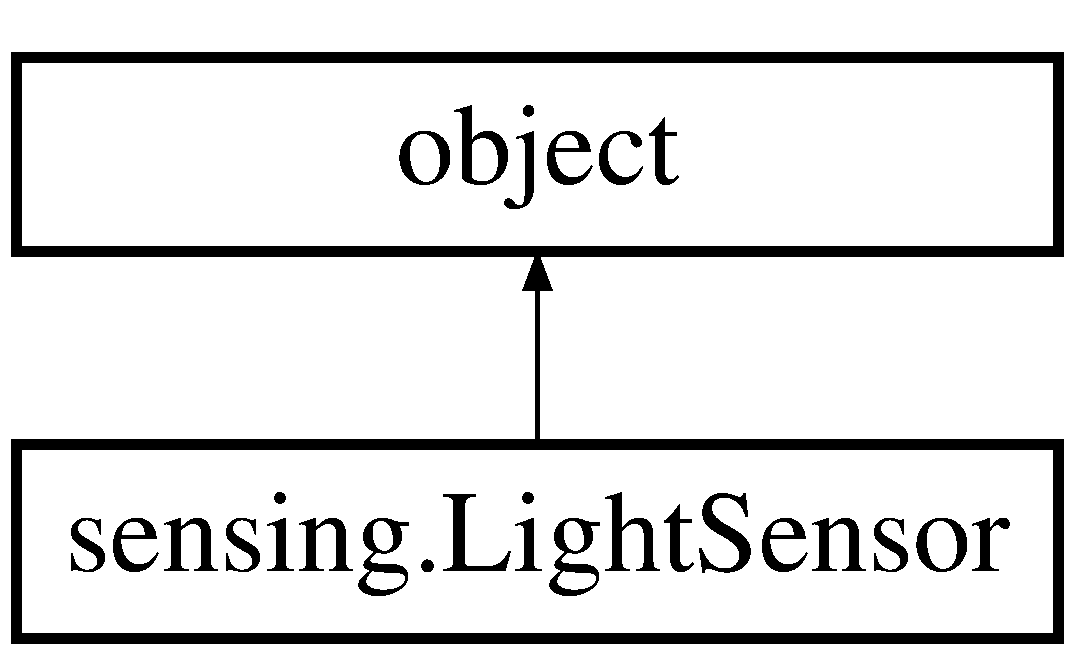
\includegraphics[height=2.000000cm]{classsensing_1_1_light_sensor}
\end{center}
\end{figure}
\subsection*{Public Member Functions}
\begin{DoxyCompactItemize}
\item 
def \hyperlink{classsensing_1_1_light_sensor_a906bcf76dc955878006f8f72dc9e3105}{\-\_\-\-\_\-init\-\_\-\-\_\-}
\begin{DoxyCompactList}\small\item\em Constructor. \end{DoxyCompactList}\item 
def \hyperlink{classsensing_1_1_light_sensor_aab3cbdaa280ccafb57e62e918940cb89}{get\-Value}
\begin{DoxyCompactList}\small\item\em This will return the sensor's name and value as a dictionary to be appended to a list of other sensors to be polled. \end{DoxyCompactList}\item 
def \hyperlink{classsensing_1_1_light_sensor_add45ebed39d38396dff214a90c6d814a}{update}
\begin{DoxyCompactList}\small\item\em The method that will read fom the pin, convert it to a value, and store that values. \end{DoxyCompactList}\item 
def \hyperlink{classsensing_1_1_light_sensor_a18d4850e295f7154bf3ff99c95c7ada6}{brightness}
\begin{DoxyCompactList}\small\item\em Because the light sensor does not truly give a readable value, we convert it to a percentage of 100. \end{DoxyCompactList}\item 
def \hyperlink{classsensing_1_1_light_sensor_aaf57806c085727f8ec922b5baa5c1f3b}{get\-Averageof\-Readings}
\begin{DoxyCompactList}\small\item\em The sensors are not perfect, so we take 5 readings and average them together before using the value. \end{DoxyCompactList}\end{DoxyCompactItemize}


\subsection{Detailed Description}
The class for a light sensor Contains all the functions to get data about the light. 

\subsection{Constructor \& Destructor Documentation}
\hypertarget{classsensing_1_1_light_sensor_a906bcf76dc955878006f8f72dc9e3105}{\index{sensing\-::\-Light\-Sensor@{sensing\-::\-Light\-Sensor}!\-\_\-\-\_\-init\-\_\-\-\_\-@{\-\_\-\-\_\-init\-\_\-\-\_\-}}
\index{\-\_\-\-\_\-init\-\_\-\-\_\-@{\-\_\-\-\_\-init\-\_\-\-\_\-}!sensing::LightSensor@{sensing\-::\-Light\-Sensor}}
\subsubsection[{\-\_\-\-\_\-init\-\_\-\-\_\-}]{\setlength{\rightskip}{0pt plus 5cm}def sensing.\-Light\-Sensor.\-\_\-\-\_\-init\-\_\-\-\_\- (
\begin{DoxyParamCaption}
\item[{}]{self, }
\item[{}]{name = {\ttfamily 'Light'}, }
\item[{}]{pin = {\ttfamily 4}}
\end{DoxyParamCaption}
)}}\label{classsensing_1_1_light_sensor_a906bcf76dc955878006f8f72dc9e3105}


Constructor. 


\begin{DoxyParams}{Parameters}
{\em name} & Optional. The name of the sensor. Defaults to \char`\"{}\-Temperature\char`\"{} \\
\hline
{\em pin} & Optional. The pin that the sensor connects through. Defaults to pin 2 \\
\hline
\end{DoxyParams}


\subsection{Member Function Documentation}
\hypertarget{classsensing_1_1_light_sensor_a18d4850e295f7154bf3ff99c95c7ada6}{\index{sensing\-::\-Light\-Sensor@{sensing\-::\-Light\-Sensor}!brightness@{brightness}}
\index{brightness@{brightness}!sensing::LightSensor@{sensing\-::\-Light\-Sensor}}
\subsubsection[{brightness}]{\setlength{\rightskip}{0pt plus 5cm}def sensing.\-Light\-Sensor.\-brightness (
\begin{DoxyParamCaption}
\item[{}]{self, }
\item[{}]{value}
\end{DoxyParamCaption}
)}}\label{classsensing_1_1_light_sensor_a18d4850e295f7154bf3ff99c95c7ada6}


Because the light sensor does not truly give a readable value, we convert it to a percentage of 100. 


\begin{DoxyParams}{Parameters}
{\em value} & The number between 0 and 4096 to convert to a percentage \\
\hline
\end{DoxyParams}
\begin{DoxyReturn}{Returns}
Will return the brightness as a percentage value 
\end{DoxyReturn}
\hypertarget{classsensing_1_1_light_sensor_aaf57806c085727f8ec922b5baa5c1f3b}{\index{sensing\-::\-Light\-Sensor@{sensing\-::\-Light\-Sensor}!get\-Averageof\-Readings@{get\-Averageof\-Readings}}
\index{get\-Averageof\-Readings@{get\-Averageof\-Readings}!sensing::LightSensor@{sensing\-::\-Light\-Sensor}}
\subsubsection[{get\-Averageof\-Readings}]{\setlength{\rightskip}{0pt plus 5cm}def sensing.\-Light\-Sensor.\-get\-Averageof\-Readings (
\begin{DoxyParamCaption}
\item[{}]{self}
\end{DoxyParamCaption}
)}}\label{classsensing_1_1_light_sensor_aaf57806c085727f8ec922b5baa5c1f3b}


The sensors are not perfect, so we take 5 readings and average them together before using the value. 

\begin{DoxyReturn}{Returns}
An average of the last 5 calculated readings 
\end{DoxyReturn}
\hypertarget{classsensing_1_1_light_sensor_aab3cbdaa280ccafb57e62e918940cb89}{\index{sensing\-::\-Light\-Sensor@{sensing\-::\-Light\-Sensor}!get\-Value@{get\-Value}}
\index{get\-Value@{get\-Value}!sensing::LightSensor@{sensing\-::\-Light\-Sensor}}
\subsubsection[{get\-Value}]{\setlength{\rightskip}{0pt plus 5cm}def sensing.\-Light\-Sensor.\-get\-Value (
\begin{DoxyParamCaption}
\item[{}]{self}
\end{DoxyParamCaption}
)}}\label{classsensing_1_1_light_sensor_aab3cbdaa280ccafb57e62e918940cb89}


This will return the sensor's name and value as a dictionary to be appended to a list of other sensors to be polled. 

\begin{DoxyReturn}{Returns}
Returns a key-\/value pair of the sensor's name in addition to the averaged value read. 
\end{DoxyReturn}
\hypertarget{classsensing_1_1_light_sensor_add45ebed39d38396dff214a90c6d814a}{\index{sensing\-::\-Light\-Sensor@{sensing\-::\-Light\-Sensor}!update@{update}}
\index{update@{update}!sensing::LightSensor@{sensing\-::\-Light\-Sensor}}
\subsubsection[{update}]{\setlength{\rightskip}{0pt plus 5cm}def sensing.\-Light\-Sensor.\-update (
\begin{DoxyParamCaption}
\item[{}]{self}
\end{DoxyParamCaption}
)}}\label{classsensing_1_1_light_sensor_add45ebed39d38396dff214a90c6d814a}


The method that will read fom the pin, convert it to a value, and store that values. 



The documentation for this class was generated from the following file\-:\begin{DoxyCompactItemize}
\item 
\hyperlink{sensing_8py}{sensing.\-py}\end{DoxyCompactItemize}

\hypertarget{classsensing_1_1_no_history_exception}{\section{sensing.\-No\-History\-Exception Class Reference}
\label{classsensing_1_1_no_history_exception}\index{sensing.\-No\-History\-Exception@{sensing.\-No\-History\-Exception}}
}


An exception that would be raised when a sensor's history list is empty.  


Inheritance diagram for sensing.\-No\-History\-Exception\-:\begin{figure}[H]
\begin{center}
\leavevmode
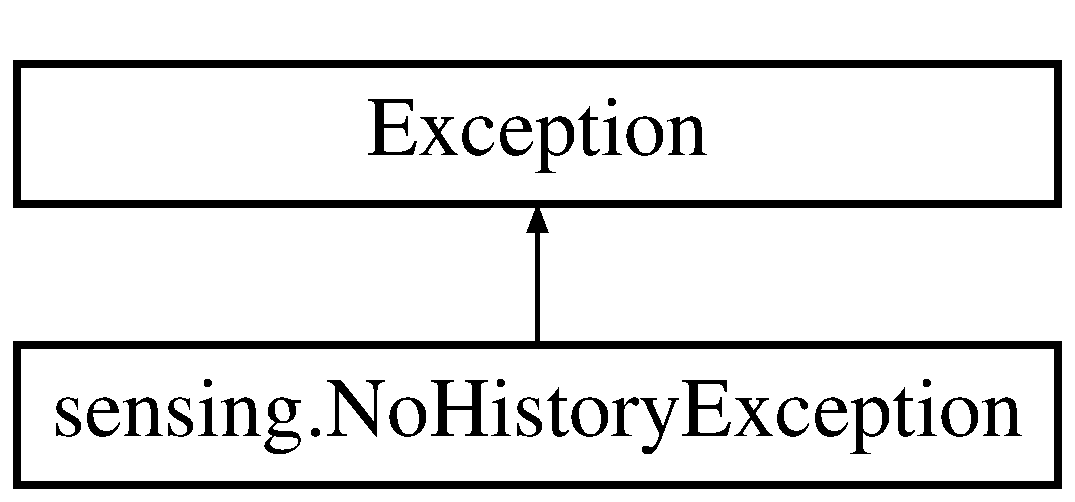
\includegraphics[height=2.000000cm]{classsensing_1_1_no_history_exception}
\end{center}
\end{figure}


\subsection{Detailed Description}
An exception that would be raised when a sensor's history list is empty. 

The documentation for this class was generated from the following file\-:\begin{DoxyCompactItemize}
\item 
\hyperlink{sensing_8py}{sensing.\-py}\end{DoxyCompactItemize}

\hypertarget{classsensing_1_1_no_pin_files_exception}{\section{sensing.\-No\-Pin\-Files\-Exception Class Reference}
\label{classsensing_1_1_no_pin_files_exception}\index{sensing.\-No\-Pin\-Files\-Exception@{sensing.\-No\-Pin\-Files\-Exception}}
}


An exception when there is no place to read Pin values from, meaning that the code is not being run on the appropriate hardware.  


Inheritance diagram for sensing.\-No\-Pin\-Files\-Exception\-:\begin{figure}[H]
\begin{center}
\leavevmode
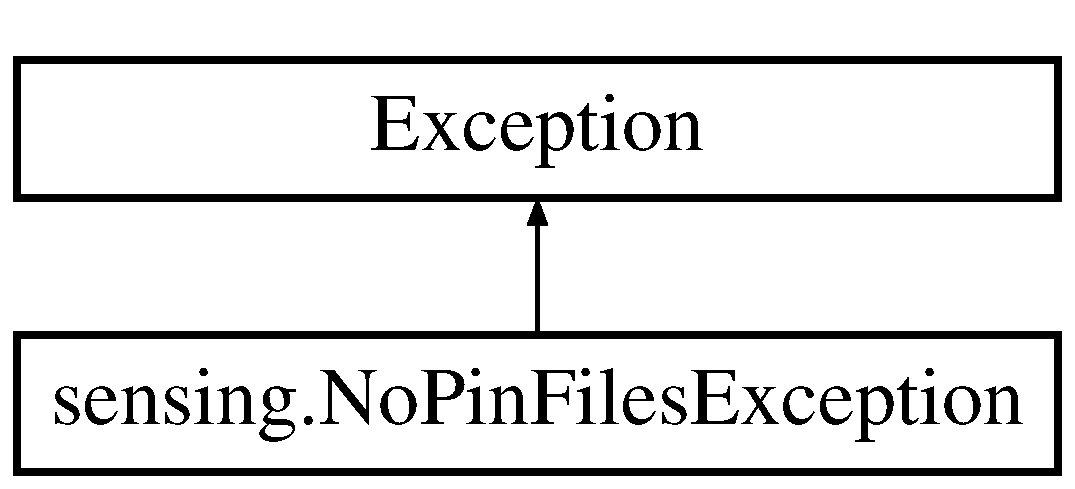
\includegraphics[height=2.000000cm]{classsensing_1_1_no_pin_files_exception}
\end{center}
\end{figure}


\subsection{Detailed Description}
An exception when there is no place to read Pin values from, meaning that the code is not being run on the appropriate hardware. 

The documentation for this class was generated from the following file\-:\begin{DoxyCompactItemize}
\item 
\hyperlink{sensing_8py}{sensing.\-py}\end{DoxyCompactItemize}

\hypertarget{classpypcduino_1_1pinmap_1_1_pin_map}{\section{pypcduino.\-pinmap.\-Pin\-Map Class Reference}
\label{classpypcduino_1_1pinmap_1_1_pin_map}\index{pypcduino.\-pinmap.\-Pin\-Map@{pypcduino.\-pinmap.\-Pin\-Map}}
}
Inheritance diagram for pypcduino.\-pinmap.\-Pin\-Map\-:\begin{figure}[H]
\begin{center}
\leavevmode
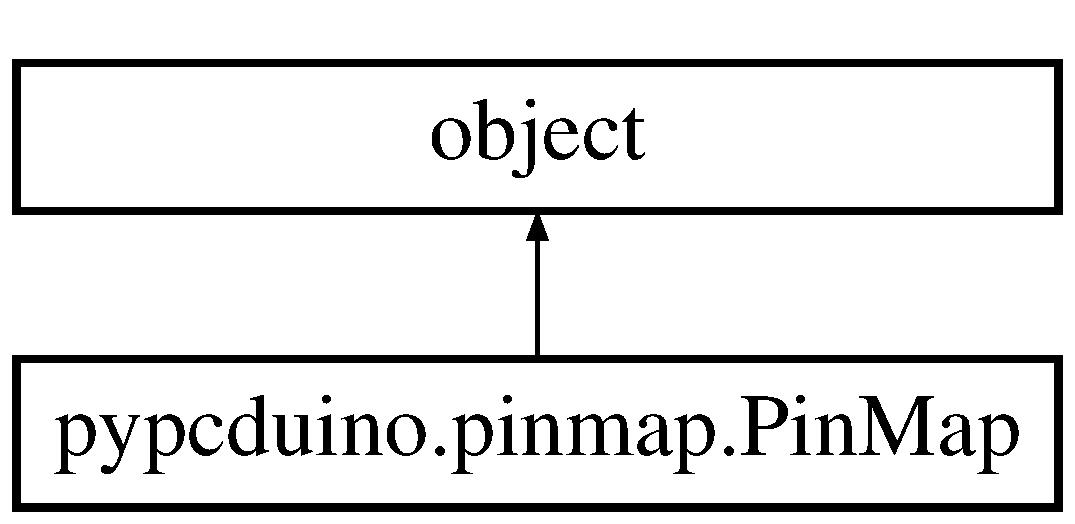
\includegraphics[height=2.000000cm]{classpypcduino_1_1pinmap_1_1_pin_map}
\end{center}
\end{figure}
\subsection*{Public Member Functions}
\begin{DoxyCompactItemize}
\item 
def \hyperlink{classpypcduino_1_1pinmap_1_1_pin_map_a712995745c0380ac734e5130b10f8d62}{\-\_\-\-\_\-init\-\_\-\-\_\-}
\item 
def \hyperlink{classpypcduino_1_1pinmap_1_1_pin_map_a64d87476c527114d9da64365d317ebf5}{get\-\_\-path}
\begin{DoxyCompactList}\small\item\em Get path of pin fd. \end{DoxyCompactList}\end{DoxyCompactItemize}
\subsection*{Public Attributes}
\begin{DoxyCompactItemize}
\item 
\hyperlink{classpypcduino_1_1pinmap_1_1_pin_map_ade5e4f0ef3667e1b1cd2fd35af39029e}{pins}
\item 
\hyperlink{classpypcduino_1_1pinmap_1_1_pin_map_a472b81fe48d6d7acbb1d4a637d870be9}{path}
\end{DoxyCompactItemize}


\subsection{Constructor \& Destructor Documentation}
\hypertarget{classpypcduino_1_1pinmap_1_1_pin_map_a712995745c0380ac734e5130b10f8d62}{\index{pypcduino\-::pinmap\-::\-Pin\-Map@{pypcduino\-::pinmap\-::\-Pin\-Map}!\-\_\-\-\_\-init\-\_\-\-\_\-@{\-\_\-\-\_\-init\-\_\-\-\_\-}}
\index{\-\_\-\-\_\-init\-\_\-\-\_\-@{\-\_\-\-\_\-init\-\_\-\-\_\-}!pypcduino::pinmap::PinMap@{pypcduino\-::pinmap\-::\-Pin\-Map}}
\subsubsection[{\-\_\-\-\_\-init\-\_\-\-\_\-}]{\setlength{\rightskip}{0pt plus 5cm}def pypcduino.\-pinmap.\-Pin\-Map.\-\_\-\-\_\-init\-\_\-\-\_\- (
\begin{DoxyParamCaption}
\item[{}]{self, }
\item[{}]{path, }
\item[{}]{prefix, }
\item[{}]{count}
\end{DoxyParamCaption}
)}}\label{classpypcduino_1_1pinmap_1_1_pin_map_a712995745c0380ac734e5130b10f8d62}


\subsection{Member Function Documentation}
\hypertarget{classpypcduino_1_1pinmap_1_1_pin_map_a64d87476c527114d9da64365d317ebf5}{\index{pypcduino\-::pinmap\-::\-Pin\-Map@{pypcduino\-::pinmap\-::\-Pin\-Map}!get\-\_\-path@{get\-\_\-path}}
\index{get\-\_\-path@{get\-\_\-path}!pypcduino::pinmap::PinMap@{pypcduino\-::pinmap\-::\-Pin\-Map}}
\subsubsection[{get\-\_\-path}]{\setlength{\rightskip}{0pt plus 5cm}def pypcduino.\-pinmap.\-Pin\-Map.\-get\-\_\-path (
\begin{DoxyParamCaption}
\item[{}]{self, }
\item[{}]{pin, }
\item[{}]{path = {\ttfamily None}}
\end{DoxyParamCaption}
)}}\label{classpypcduino_1_1pinmap_1_1_pin_map_a64d87476c527114d9da64365d317ebf5}


Get path of pin fd. 

pin can either be the pin basename (i.\-e. 'adc2') or pin number (i.\-e. 2) if prefix is supplied, override the default path prefix. 

\subsection{Member Data Documentation}
\hypertarget{classpypcduino_1_1pinmap_1_1_pin_map_a472b81fe48d6d7acbb1d4a637d870be9}{\index{pypcduino\-::pinmap\-::\-Pin\-Map@{pypcduino\-::pinmap\-::\-Pin\-Map}!path@{path}}
\index{path@{path}!pypcduino::pinmap::PinMap@{pypcduino\-::pinmap\-::\-Pin\-Map}}
\subsubsection[{path}]{\setlength{\rightskip}{0pt plus 5cm}pypcduino.\-pinmap.\-Pin\-Map.\-path}}\label{classpypcduino_1_1pinmap_1_1_pin_map_a472b81fe48d6d7acbb1d4a637d870be9}
\hypertarget{classpypcduino_1_1pinmap_1_1_pin_map_ade5e4f0ef3667e1b1cd2fd35af39029e}{\index{pypcduino\-::pinmap\-::\-Pin\-Map@{pypcduino\-::pinmap\-::\-Pin\-Map}!pins@{pins}}
\index{pins@{pins}!pypcduino::pinmap::PinMap@{pypcduino\-::pinmap\-::\-Pin\-Map}}
\subsubsection[{pins}]{\setlength{\rightskip}{0pt plus 5cm}pypcduino.\-pinmap.\-Pin\-Map.\-pins}}\label{classpypcduino_1_1pinmap_1_1_pin_map_ade5e4f0ef3667e1b1cd2fd35af39029e}


The documentation for this class was generated from the following file\-:\begin{DoxyCompactItemize}
\item 
/home/justin/\-C\-S\-C\-I\-Project/pcduino/pypcduino/\hyperlink{pinmap_8py}{pinmap.\-py}\end{DoxyCompactItemize}

\hypertarget{classsensing_1_1_pin_read_out_of_range_exception}{\section{sensing.\-Pin\-Read\-Out\-Of\-Range\-Exception Class Reference}
\label{classsensing_1_1_pin_read_out_of_range_exception}\index{sensing.\-Pin\-Read\-Out\-Of\-Range\-Exception@{sensing.\-Pin\-Read\-Out\-Of\-Range\-Exception}}
}


An exception that should occur when a pin reads out of range (0-\/4096)  


Inheritance diagram for sensing.\-Pin\-Read\-Out\-Of\-Range\-Exception\-:\begin{figure}[H]
\begin{center}
\leavevmode
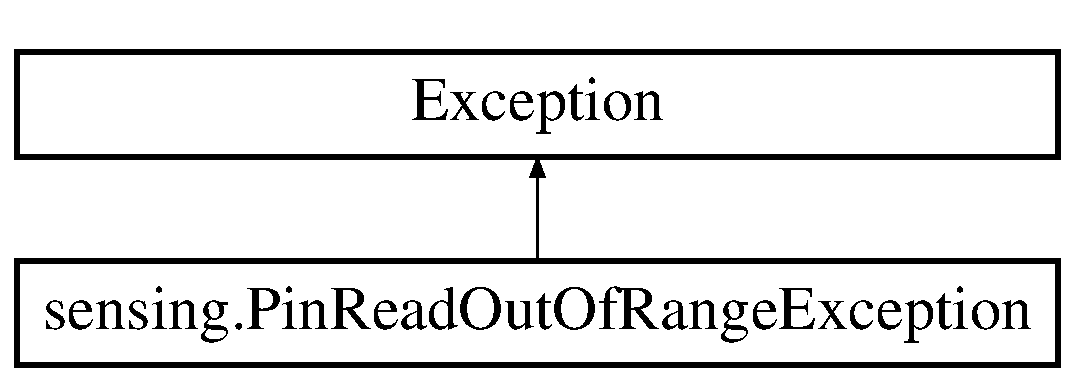
\includegraphics[height=2.000000cm]{classsensing_1_1_pin_read_out_of_range_exception}
\end{center}
\end{figure}


\subsection{Detailed Description}
An exception that should occur when a pin reads out of range (0-\/4096) 

The documentation for this class was generated from the following file\-:\begin{DoxyCompactItemize}
\item 
\hyperlink{sensing_8py}{sensing.\-py}\end{DoxyCompactItemize}

\hypertarget{classsensing_1_1_sensor_name_exception}{\section{sensing.\-Sensor\-Name\-Exception Class Reference}
\label{classsensing_1_1_sensor_name_exception}\index{sensing.\-Sensor\-Name\-Exception@{sensing.\-Sensor\-Name\-Exception}}
}


An exception to get thrown when a sensor was set up with an invalid name.  


Inheritance diagram for sensing.\-Sensor\-Name\-Exception\-:\begin{figure}[H]
\begin{center}
\leavevmode
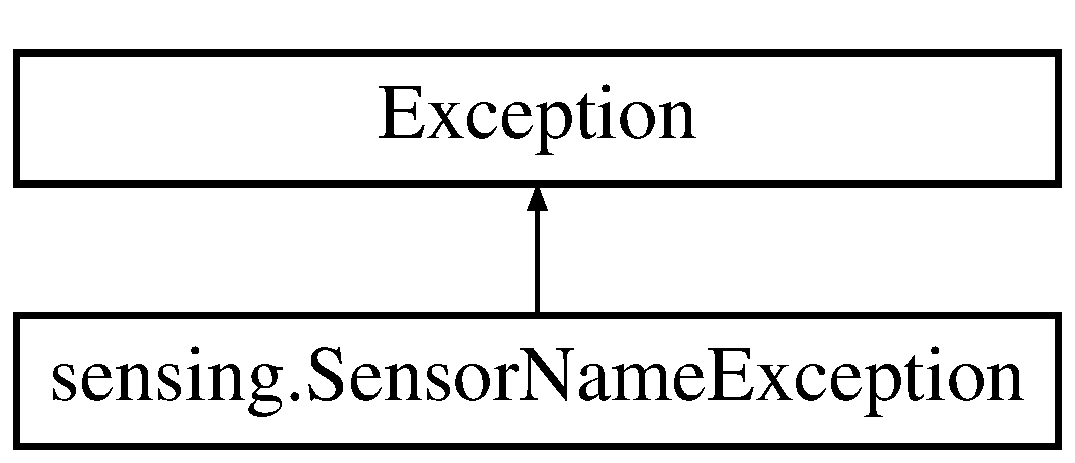
\includegraphics[height=2.000000cm]{classsensing_1_1_sensor_name_exception}
\end{center}
\end{figure}


\subsection{Detailed Description}
An exception to get thrown when a sensor was set up with an invalid name. 

The documentation for this class was generated from the following file\-:\begin{DoxyCompactItemize}
\item 
\hyperlink{sensing_8py}{sensing.\-py}\end{DoxyCompactItemize}

\hypertarget{classsensing_1_1_sensor_pin_exception}{\section{sensing.\-Sensor\-Pin\-Exception Class Reference}
\label{classsensing_1_1_sensor_pin_exception}\index{sensing.\-Sensor\-Pin\-Exception@{sensing.\-Sensor\-Pin\-Exception}}
}


An exception to get thrown when a sensor was set up with an invalid pin location.  


Inheritance diagram for sensing.\-Sensor\-Pin\-Exception\-:\begin{figure}[H]
\begin{center}
\leavevmode
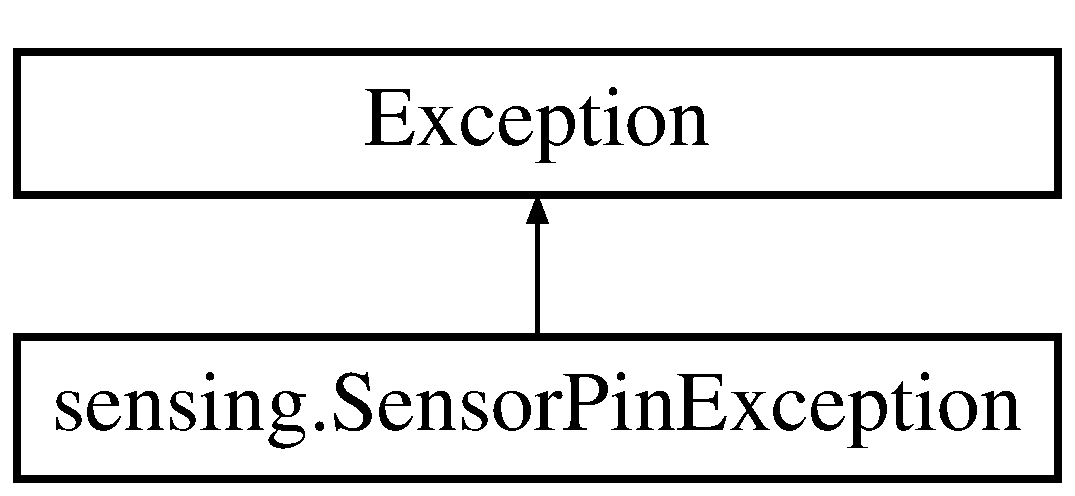
\includegraphics[height=2.000000cm]{classsensing_1_1_sensor_pin_exception}
\end{center}
\end{figure}


\subsection{Detailed Description}
An exception to get thrown when a sensor was set up with an invalid pin location. 

The documentation for this class was generated from the following file\-:\begin{DoxyCompactItemize}
\item 
/home/justin/\-C\-S\-C\-I\-Project/pcduino/\hyperlink{sensing_8py}{sensing.\-py}\end{DoxyCompactItemize}

\hypertarget{classsensing_1_1_temperature_sensor}{\section{sensing.\-Temperature\-Sensor Class Reference}
\label{classsensing_1_1_temperature_sensor}\index{sensing.\-Temperature\-Sensor@{sensing.\-Temperature\-Sensor}}
}


The class for a Temperature Sensor It has the functions to get the temperature and parse it.  


Inheritance diagram for sensing.\-Temperature\-Sensor\-:\begin{figure}[H]
\begin{center}
\leavevmode
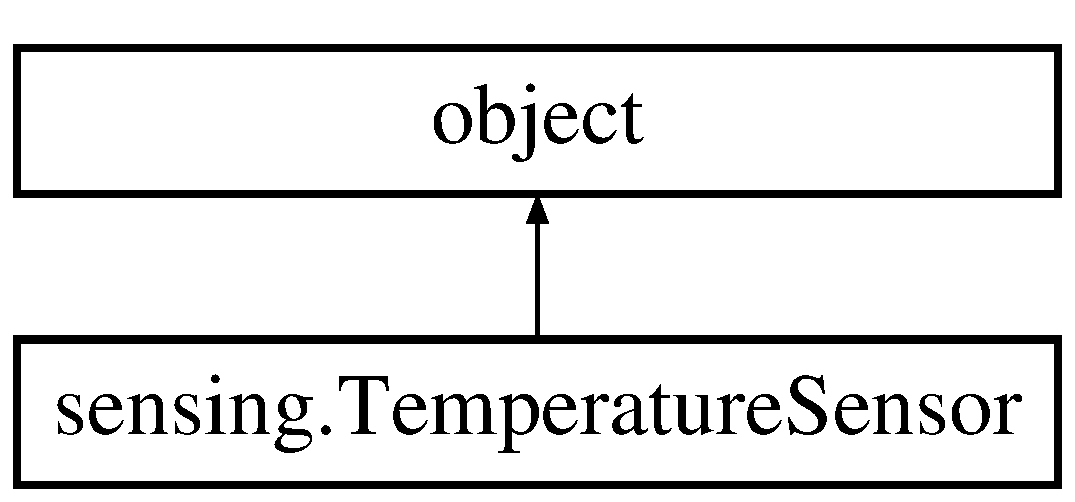
\includegraphics[height=2.000000cm]{classsensing_1_1_temperature_sensor}
\end{center}
\end{figure}
\subsection*{Public Member Functions}
\begin{DoxyCompactItemize}
\item 
def \hyperlink{classsensing_1_1_temperature_sensor_a35bf393ac9f3fadc1bcec9e32eb9a7d6}{\-\_\-\-\_\-init\-\_\-\-\_\-}
\begin{DoxyCompactList}\small\item\em The constructor, which sets the name of the sensor for the server and which pin needs to be polled. \end{DoxyCompactList}\item 
def \hyperlink{classsensing_1_1_temperature_sensor_aaeb85a07038568c56f0e3543815068d7}{ad\-To\-Voltage}
\begin{DoxyCompactList}\small\item\em The reading from the board is not formatted in the correct units, so we first need to find what the millivoltage that the board is reading is. \end{DoxyCompactList}\item 
def \hyperlink{classsensing_1_1_temperature_sensor_a5129c7aa8fabc66c80b645186518ecac}{get\-Averageof\-Readings}
\begin{DoxyCompactList}\small\item\em The sensors are not perfect, so we take 5 readings and average them together before using the value. \end{DoxyCompactList}\item 
def \hyperlink{classsensing_1_1_temperature_sensor_aaf6d138cf7d3155597a11b359fa9afe7}{voltage\-To\-Temp}
\begin{DoxyCompactList}\small\item\em We need to convert the millivoltage to an actual temperature. \end{DoxyCompactList}\item 
def \hyperlink{classsensing_1_1_temperature_sensor_adce48cedf1d9fdd706c374ec1217bd94}{update}
\begin{DoxyCompactList}\small\item\em The method that will read fom the pin, convert it to a value, and store that value 
\begin{DoxyExceptions}{Exceptions}
{\em Pin\-Read\-Outof\-Range\-Exception} & Will be thrown when the reading we get is out of the acceptable range. \\
\hline
\end{DoxyExceptions}
\end{DoxyCompactList}\item 
def \hyperlink{classsensing_1_1_temperature_sensor_a556e30e17858efbb95521dfafe6ee0cc}{get\-Value}
\begin{DoxyCompactList}\small\item\em This will return the sensor's name and value as a dictionary to be appended to a list of other sensors to be polled. \end{DoxyCompactList}\end{DoxyCompactItemize}


\subsection{Detailed Description}
The class for a Temperature Sensor It has the functions to get the temperature and parse it. 

\subsection{Constructor \& Destructor Documentation}
\hypertarget{classsensing_1_1_temperature_sensor_a35bf393ac9f3fadc1bcec9e32eb9a7d6}{\index{sensing\-::\-Temperature\-Sensor@{sensing\-::\-Temperature\-Sensor}!\-\_\-\-\_\-init\-\_\-\-\_\-@{\-\_\-\-\_\-init\-\_\-\-\_\-}}
\index{\-\_\-\-\_\-init\-\_\-\-\_\-@{\-\_\-\-\_\-init\-\_\-\-\_\-}!sensing::TemperatureSensor@{sensing\-::\-Temperature\-Sensor}}
\subsubsection[{\-\_\-\-\_\-init\-\_\-\-\_\-}]{\setlength{\rightskip}{0pt plus 5cm}def sensing.\-Temperature\-Sensor.\-\_\-\-\_\-init\-\_\-\-\_\- (
\begin{DoxyParamCaption}
\item[{}]{self, }
\item[{}]{name = {\ttfamily 'Temperature'}, }
\item[{}]{pin = {\ttfamily 2}}
\end{DoxyParamCaption}
)}}\label{classsensing_1_1_temperature_sensor_a35bf393ac9f3fadc1bcec9e32eb9a7d6}


The constructor, which sets the name of the sensor for the server and which pin needs to be polled. 


\begin{DoxyParams}{Parameters}
{\em name} & Optional. The name of the sensor. Defaults to \char`\"{}\-Temperature\char`\"{} \\
\hline
{\em pin} & Optional. The pin that the sensor connects through. Defaults to pin 2 \\
\hline
\end{DoxyParams}

\begin{DoxyExceptions}{Exceptions}
{\em \hyperlink{classsensing_1_1_sensor_pin_exception}{Sensor\-Pin\-Exception}} & Thrown when the pin specified is not in the valid range \\
\hline
\end{DoxyExceptions}


\subsection{Member Function Documentation}
\hypertarget{classsensing_1_1_temperature_sensor_aaeb85a07038568c56f0e3543815068d7}{\index{sensing\-::\-Temperature\-Sensor@{sensing\-::\-Temperature\-Sensor}!ad\-To\-Voltage@{ad\-To\-Voltage}}
\index{ad\-To\-Voltage@{ad\-To\-Voltage}!sensing::TemperatureSensor@{sensing\-::\-Temperature\-Sensor}}
\subsubsection[{ad\-To\-Voltage}]{\setlength{\rightskip}{0pt plus 5cm}def sensing.\-Temperature\-Sensor.\-ad\-To\-Voltage (
\begin{DoxyParamCaption}
\item[{}]{self}
\end{DoxyParamCaption}
)}}\label{classsensing_1_1_temperature_sensor_aaeb85a07038568c56f0e3543815068d7}


The reading from the board is not formatted in the correct units, so we first need to find what the millivoltage that the board is reading is. 

\begin{DoxyReturn}{Returns}
Returns the A\-D reading as a calculated voltage 
\end{DoxyReturn}
\hypertarget{classsensing_1_1_temperature_sensor_a5129c7aa8fabc66c80b645186518ecac}{\index{sensing\-::\-Temperature\-Sensor@{sensing\-::\-Temperature\-Sensor}!get\-Averageof\-Readings@{get\-Averageof\-Readings}}
\index{get\-Averageof\-Readings@{get\-Averageof\-Readings}!sensing::TemperatureSensor@{sensing\-::\-Temperature\-Sensor}}
\subsubsection[{get\-Averageof\-Readings}]{\setlength{\rightskip}{0pt plus 5cm}def sensing.\-Temperature\-Sensor.\-get\-Averageof\-Readings (
\begin{DoxyParamCaption}
\item[{}]{self}
\end{DoxyParamCaption}
)}}\label{classsensing_1_1_temperature_sensor_a5129c7aa8fabc66c80b645186518ecac}


The sensors are not perfect, so we take 5 readings and average them together before using the value. 

\begin{DoxyReturn}{Returns}
An average of the last 5 calculated readings 
\end{DoxyReturn}

\begin{DoxyExceptions}{Exceptions}
{\em \hyperlink{classsensing_1_1_no_history_exception}{No\-History\-Exception}} & Thrown when there are no readings in the history. \\
\hline
\end{DoxyExceptions}
\hypertarget{classsensing_1_1_temperature_sensor_a556e30e17858efbb95521dfafe6ee0cc}{\index{sensing\-::\-Temperature\-Sensor@{sensing\-::\-Temperature\-Sensor}!get\-Value@{get\-Value}}
\index{get\-Value@{get\-Value}!sensing::TemperatureSensor@{sensing\-::\-Temperature\-Sensor}}
\subsubsection[{get\-Value}]{\setlength{\rightskip}{0pt plus 5cm}def sensing.\-Temperature\-Sensor.\-get\-Value (
\begin{DoxyParamCaption}
\item[{}]{self}
\end{DoxyParamCaption}
)}}\label{classsensing_1_1_temperature_sensor_a556e30e17858efbb95521dfafe6ee0cc}


This will return the sensor's name and value as a dictionary to be appended to a list of other sensors to be polled. 

\begin{DoxyReturn}{Returns}
Returns a key-\/value pair of the sensor's name in addition to the averaged value read. 
\end{DoxyReturn}
\hypertarget{classsensing_1_1_temperature_sensor_adce48cedf1d9fdd706c374ec1217bd94}{\index{sensing\-::\-Temperature\-Sensor@{sensing\-::\-Temperature\-Sensor}!update@{update}}
\index{update@{update}!sensing::TemperatureSensor@{sensing\-::\-Temperature\-Sensor}}
\subsubsection[{update}]{\setlength{\rightskip}{0pt plus 5cm}def sensing.\-Temperature\-Sensor.\-update (
\begin{DoxyParamCaption}
\item[{}]{self}
\end{DoxyParamCaption}
)}}\label{classsensing_1_1_temperature_sensor_adce48cedf1d9fdd706c374ec1217bd94}


The method that will read fom the pin, convert it to a value, and store that value 
\begin{DoxyExceptions}{Exceptions}
{\em Pin\-Read\-Outof\-Range\-Exception} & Will be thrown when the reading we get is out of the acceptable range. \\
\hline
\end{DoxyExceptions}


\hypertarget{classsensing_1_1_temperature_sensor_aaf6d138cf7d3155597a11b359fa9afe7}{\index{sensing\-::\-Temperature\-Sensor@{sensing\-::\-Temperature\-Sensor}!voltage\-To\-Temp@{voltage\-To\-Temp}}
\index{voltage\-To\-Temp@{voltage\-To\-Temp}!sensing::TemperatureSensor@{sensing\-::\-Temperature\-Sensor}}
\subsubsection[{voltage\-To\-Temp}]{\setlength{\rightskip}{0pt plus 5cm}def sensing.\-Temperature\-Sensor.\-voltage\-To\-Temp (
\begin{DoxyParamCaption}
\item[{}]{self, }
\item[{}]{voltage}
\end{DoxyParamCaption}
)}}\label{classsensing_1_1_temperature_sensor_aaf6d138cf7d3155597a11b359fa9afe7}


We need to convert the millivoltage to an actual temperature. 


\begin{DoxyParams}{Parameters}
{\em voltage} & The voltage to convert \\
\hline
\end{DoxyParams}
\begin{DoxyReturn}{Returns}
Calculated Fahrenheit temperature from the voltage 
\end{DoxyReturn}


The documentation for this class was generated from the following file\-:\begin{DoxyCompactItemize}
\item 
\hyperlink{sensing_8py}{sensing.\-py}\end{DoxyCompactItemize}

\hypertarget{classtest__sensing_1_1_test_sensing}{\section{test\-\_\-sensing.\-Test\-Sensing Class Reference}
\label{classtest__sensing_1_1_test_sensing}\index{test\-\_\-sensing.\-Test\-Sensing@{test\-\_\-sensing.\-Test\-Sensing}}
}
Inheritance diagram for test\-\_\-sensing.\-Test\-Sensing\-:\begin{figure}[H]
\begin{center}
\leavevmode
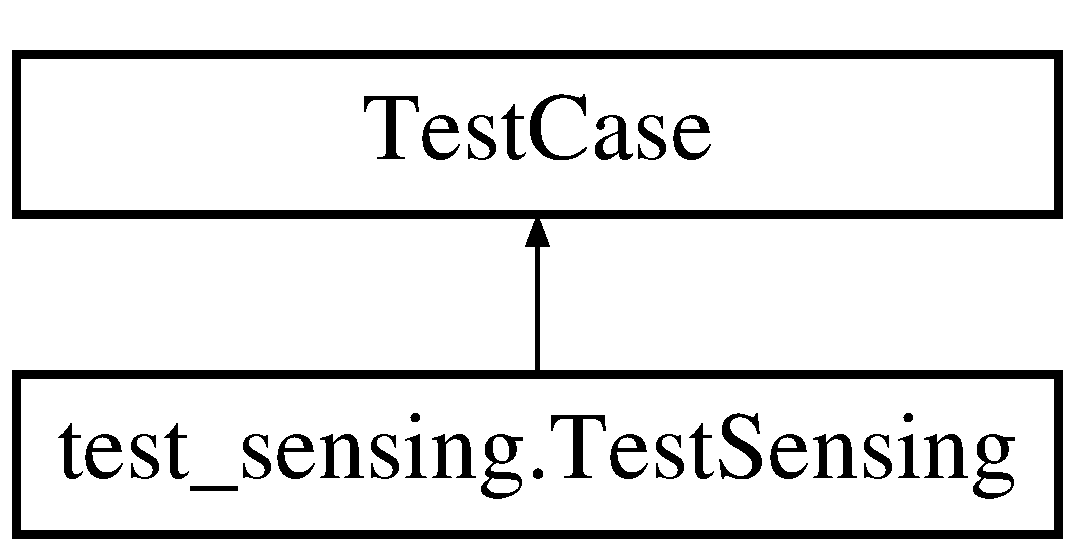
\includegraphics[height=2.000000cm]{classtest__sensing_1_1_test_sensing}
\end{center}
\end{figure}
\subsection*{Public Member Functions}
\begin{DoxyCompactItemize}
\item 
def \hyperlink{classtest__sensing_1_1_test_sensing_a8108831848700c03f289e756d849268b}{setup}
\item 
def \hyperlink{classtest__sensing_1_1_test_sensing_a0d1b334a31f4dea05ffd10d032069bd6}{test\-\_\-\-Light\-Sensor}
\item 
def \hyperlink{classtest__sensing_1_1_test_sensing_ac31ab35d2d8ef9a50d0e87f340334450}{test\-\_\-\-Temp\-Sensor}
\end{DoxyCompactItemize}


\subsection{Member Function Documentation}
\hypertarget{classtest__sensing_1_1_test_sensing_a8108831848700c03f289e756d849268b}{\index{test\-\_\-sensing\-::\-Test\-Sensing@{test\-\_\-sensing\-::\-Test\-Sensing}!setup@{setup}}
\index{setup@{setup}!test_sensing::TestSensing@{test\-\_\-sensing\-::\-Test\-Sensing}}
\subsubsection[{setup}]{\setlength{\rightskip}{0pt plus 5cm}def test\-\_\-sensing.\-Test\-Sensing.\-setup (
\begin{DoxyParamCaption}
\item[{}]{self}
\end{DoxyParamCaption}
)}}\label{classtest__sensing_1_1_test_sensing_a8108831848700c03f289e756d849268b}
\hypertarget{classtest__sensing_1_1_test_sensing_a0d1b334a31f4dea05ffd10d032069bd6}{\index{test\-\_\-sensing\-::\-Test\-Sensing@{test\-\_\-sensing\-::\-Test\-Sensing}!test\-\_\-\-Light\-Sensor@{test\-\_\-\-Light\-Sensor}}
\index{test\-\_\-\-Light\-Sensor@{test\-\_\-\-Light\-Sensor}!test_sensing::TestSensing@{test\-\_\-sensing\-::\-Test\-Sensing}}
\subsubsection[{test\-\_\-\-Light\-Sensor}]{\setlength{\rightskip}{0pt plus 5cm}def test\-\_\-sensing.\-Test\-Sensing.\-test\-\_\-\-Light\-Sensor (
\begin{DoxyParamCaption}
\item[{}]{self}
\end{DoxyParamCaption}
)}}\label{classtest__sensing_1_1_test_sensing_a0d1b334a31f4dea05ffd10d032069bd6}
\hypertarget{classtest__sensing_1_1_test_sensing_ac31ab35d2d8ef9a50d0e87f340334450}{\index{test\-\_\-sensing\-::\-Test\-Sensing@{test\-\_\-sensing\-::\-Test\-Sensing}!test\-\_\-\-Temp\-Sensor@{test\-\_\-\-Temp\-Sensor}}
\index{test\-\_\-\-Temp\-Sensor@{test\-\_\-\-Temp\-Sensor}!test_sensing::TestSensing@{test\-\_\-sensing\-::\-Test\-Sensing}}
\subsubsection[{test\-\_\-\-Temp\-Sensor}]{\setlength{\rightskip}{0pt plus 5cm}def test\-\_\-sensing.\-Test\-Sensing.\-test\-\_\-\-Temp\-Sensor (
\begin{DoxyParamCaption}
\item[{}]{self}
\end{DoxyParamCaption}
)}}\label{classtest__sensing_1_1_test_sensing_ac31ab35d2d8ef9a50d0e87f340334450}


The documentation for this class was generated from the following file\-:\begin{DoxyCompactItemize}
\item 
/home/justin/\-C\-S\-C\-I\-Project/pcduino/\hyperlink{test__sensing_8py}{test\-\_\-sensing.\-py}\end{DoxyCompactItemize}

\chapter{File Documentation}
\hypertarget{____init_____8py}{\section{pypcduino/\-\_\-\-\_\-init\-\_\-\-\_\-.py File Reference}
\label{____init_____8py}\index{pypcduino/\-\_\-\-\_\-init\-\_\-\-\_\-.\-py@{pypcduino/\-\_\-\-\_\-init\-\_\-\-\_\-.\-py}}
}
\subsection*{Namespaces}
\begin{DoxyCompactItemize}
\item 
\hyperlink{namespacepypcduino}{pypcduino}
\end{DoxyCompactItemize}

\hypertarget{adc_8py}{\section{pypcduino/adc.py File Reference}
\label{adc_8py}\index{pypcduino/adc.\-py@{pypcduino/adc.\-py}}
}
\subsection*{Namespaces}
\begin{DoxyCompactItemize}
\item 
\hyperlink{namespacepypcduino_1_1adc}{pypcduino.\-adc}
\end{DoxyCompactItemize}
\subsection*{Functions}
\begin{DoxyCompactItemize}
\item 
def \hyperlink{namespacepypcduino_1_1adc_a3ef1a506a5cb668cf5b418c804facbcd}{pypcduino.\-adc.\-analog\-\_\-read}
\begin{DoxyCompactList}\small\item\em Return the integer value of an adc pin. \end{DoxyCompactList}\end{DoxyCompactItemize}
\subsection*{Variables}
\begin{DoxyCompactItemize}
\item 
tuple \hyperlink{namespacepypcduino_1_1adc_a766105e33e35d9fa020e87c19e6ddf07}{pypcduino.\-adc.\-pins} = Pin\-Map('/proc', 'adc', 6)
\end{DoxyCompactItemize}

\hypertarget{exceptions_8py}{\section{/home/justin/\-C\-S\-C\-I\-Project/pcduino/pypcduino/exceptions.py File Reference}
\label{exceptions_8py}\index{/home/justin/\-C\-S\-C\-I\-Project/pcduino/pypcduino/exceptions.\-py@{/home/justin/\-C\-S\-C\-I\-Project/pcduino/pypcduino/exceptions.\-py}}
}
\subsection*{Namespaces}
\begin{DoxyCompactItemize}
\item 
\hyperlink{namespacepypcduino_1_1exceptions}{pypcduino.\-exceptions}
\end{DoxyCompactItemize}

\hypertarget{gpio_8py}{\section{/home/justin/\-C\-S\-C\-I\-Project/pcduino/pypcduino/gpio.py File Reference}
\label{gpio_8py}\index{/home/justin/\-C\-S\-C\-I\-Project/pcduino/pypcduino/gpio.\-py@{/home/justin/\-C\-S\-C\-I\-Project/pcduino/pypcduino/gpio.\-py}}
}
\subsection*{Namespaces}
\begin{DoxyCompactItemize}
\item 
\hyperlink{namespacepypcduino_1_1gpio}{pypcduino.\-gpio}
\end{DoxyCompactItemize}
\subsection*{Functions}
\begin{DoxyCompactItemize}
\item 
def \hyperlink{namespacepypcduino_1_1gpio_aba7c287e8da39dc2e5f7951ebe7819a4}{pypcduino.\-gpio.\-digital\-\_\-write}
\begin{DoxyCompactList}\small\item\em Write to a G\-P\-I\-O channel. \end{DoxyCompactList}\item 
def \hyperlink{namespacepypcduino_1_1gpio_aa324a331fb50643f94e222b8eef38fe8}{pypcduino.\-gpio.\-digital\-\_\-read}
\begin{DoxyCompactList}\small\item\em Read from a G\-P\-I\-O channel. \end{DoxyCompactList}\item 
def \hyperlink{namespacepypcduino_1_1gpio_af0917a2382b59c8825b60df9cc4d6830}{pypcduino.\-gpio.\-pin\-\_\-mode}
\begin{DoxyCompactList}\small\item\em Set Mode of a G\-P\-I\-O channel. \end{DoxyCompactList}\end{DoxyCompactItemize}
\subsection*{Variables}
\begin{DoxyCompactItemize}
\item 
list \hyperlink{namespacepypcduino_1_1gpio_a8a55cdc8c6b775ffa9ba8aa68cfd8d93}{pypcduino.\-gpio.\-\_\-\-\_\-all\-\_\-\-\_\-}
\item 
int \hyperlink{namespacepypcduino_1_1gpio_a017380b78afe9853e0cc3ca009c47ec3}{pypcduino.\-gpio.\-H\-I\-G\-H} = 1
\item 
int \hyperlink{namespacepypcduino_1_1gpio_a7794534b6aba1a94e2ed468ec8fbed98}{pypcduino.\-gpio.\-L\-O\-W} = 0
\item 
int \hyperlink{namespacepypcduino_1_1gpio_afabe8a2ce86d5db92f8e5994e5c24252}{pypcduino.\-gpio.\-I\-N\-P\-U\-T} = 0
\item 
int \hyperlink{namespacepypcduino_1_1gpio_a810c8642dc31f28d747c4c845e8a4a80}{pypcduino.\-gpio.\-O\-U\-T\-P\-U\-T} = 1
\item 
tuple \hyperlink{namespacepypcduino_1_1gpio_acf2dcb151997749e99dbf65c08073e08}{pypcduino.\-gpio.\-gpio\-\_\-pins}
\item 
tuple \hyperlink{namespacepypcduino_1_1gpio_a3e40fb727c6bb0d0f1bcf69478a9a1c0}{pypcduino.\-gpio.\-gpio\-\_\-mode\-\_\-pins}
\end{DoxyCompactItemize}

\hypertarget{pinmap_8py}{\section{pypcduino/pinmap.py File Reference}
\label{pinmap_8py}\index{pypcduino/pinmap.\-py@{pypcduino/pinmap.\-py}}
}
\subsection*{Classes}
\begin{DoxyCompactItemize}
\item 
class \hyperlink{classpypcduino_1_1pinmap_1_1_invalid_channel_exception}{pypcduino.\-pinmap.\-Invalid\-Channel\-Exception}
\begin{DoxyCompactList}\small\item\em The channel sent was invalid. \end{DoxyCompactList}\item 
class \hyperlink{classpypcduino_1_1pinmap_1_1_pin_map}{pypcduino.\-pinmap.\-Pin\-Map}
\end{DoxyCompactItemize}
\subsection*{Namespaces}
\begin{DoxyCompactItemize}
\item 
\hyperlink{namespacepypcduino_1_1pinmap}{pypcduino.\-pinmap}
\end{DoxyCompactItemize}

\hypertarget{sensing_8py}{\section{sensing.\-py File Reference}
\label{sensing_8py}\index{sensing.\-py@{sensing.\-py}}
}
\subsection*{Classes}
\begin{DoxyCompactItemize}
\item 
class \hyperlink{classsensing_1_1_temperature_sensor}{sensing.\-Temperature\-Sensor}
\begin{DoxyCompactList}\small\item\em The class for a Temperature Sensor It has the functions to get the temperature and parse it. \end{DoxyCompactList}\item 
class \hyperlink{classsensing_1_1_light_sensor}{sensing.\-Light\-Sensor}
\begin{DoxyCompactList}\small\item\em The class for a light sensor Contains all the functions to get data about the light. \end{DoxyCompactList}\item 
class \hyperlink{classsensing_1_1_sensor_pin_exception}{sensing.\-Sensor\-Pin\-Exception}
\begin{DoxyCompactList}\small\item\em An exception to get thrown when a sensor was set up with an invalid pin location. \end{DoxyCompactList}\item 
class \hyperlink{classsensing_1_1_sensor_name_exception}{sensing.\-Sensor\-Name\-Exception}
\begin{DoxyCompactList}\small\item\em An exception to get thrown when a sensor was set up with an invalid name. \end{DoxyCompactList}\item 
class \hyperlink{classsensing_1_1_no_history_exception}{sensing.\-No\-History\-Exception}
\begin{DoxyCompactList}\small\item\em An exception that would be raised when a sensor's history list is empty. \end{DoxyCompactList}\item 
class \hyperlink{classsensing_1_1_pin_read_out_of_range_exception}{sensing.\-Pin\-Read\-Out\-Of\-Range\-Exception}
\begin{DoxyCompactList}\small\item\em An exception that should occur when a pin reads out of range (0-\/4096) \end{DoxyCompactList}\item 
class \hyperlink{classsensing_1_1_no_pin_files_exception}{sensing.\-No\-Pin\-Files\-Exception}
\begin{DoxyCompactList}\small\item\em An exception when there is no place to read Pin values from, meaning that the code is not being run on the appropriate hardware. \end{DoxyCompactList}\end{DoxyCompactItemize}
\subsection*{Namespaces}
\begin{DoxyCompactItemize}
\item 
\hyperlink{namespacesensing}{sensing}
\end{DoxyCompactItemize}
\subsection*{Functions}
\begin{DoxyCompactItemize}
\item 
def \hyperlink{namespacesensing_a110922c2a80aabf038d162595e137cc4}{sensing.\-delay}
\begin{DoxyCompactList}\small\item\em Put the program to sleep for a specified number of milliseconds. \end{DoxyCompactList}\item 
def \hyperlink{namespacesensing_afc4f85f529614a384ee1d04cd5ff80f3}{sensing.\-loop}
\begin{DoxyCompactList}\small\item\em The main loop. \end{DoxyCompactList}\item 
def \hyperlink{namespacesensing_aeae2450fef0f1a9244c1ddc6d96ef4c2}{sensing.\-send\-Data}
\begin{DoxyCompactList}\small\item\em Here we actually ship off the information to the server. \end{DoxyCompactList}\item 
def \hyperlink{namespacesensing_a75479ff0f15da4027d590f94160bb43f}{sensing.\-update\-Pin\-Readings}
\begin{DoxyCompactList}\small\item\em This function will read the values reported by the hardware, and then save that data to the appropriate sensor's variable. \end{DoxyCompactList}\item 
def \hyperlink{namespacesensing_af9472a5ce179d5f4cbbc2d02a9dbed14}{sensing.\-get\-Sensor\-Data}
\begin{DoxyCompactList}\small\item\em This function will retrieve the averaged values from the sensors and format it into a dictionary. \end{DoxyCompactList}\item 
def \hyperlink{namespacesensing_a3b1d400f9ad84146d60ee62f7e82faa0}{sensing.\-setup\-Sensors}
\begin{DoxyCompactList}\small\item\em Any sensors that are available will be added to a list that gets polled later for their readings. \end{DoxyCompactList}\item 
def \hyperlink{namespacesensing_a38d7f8a9b27bbcf471a89725a5e78493}{sensing.\-main}
\begin{DoxyCompactList}\small\item\em The entry point of the program, where we will make a call to setup the various connected sensors, and then begin looping indefinitely to poll those sensors and upload the collected data. \end{DoxyCompactList}\end{DoxyCompactItemize}
\subsection*{Variables}
\begin{DoxyCompactItemize}
\item 
string \hyperlink{namespacesensing_a7d59d9b021482661d93cbf2120dfa030}{sensing.\-board\-Name} = ''
\begin{DoxyCompactList}\small\item\em The I\-D/tag to identify the individual board, passed as a command-\/line argument. \end{DoxyCompactList}\item 
list \hyperlink{namespacesensing_a46ffa95be1accb04ea0a2c0b89b217c0}{sensing.\-available\-Sensors} = \mbox{[}$\,$\mbox{]}
\begin{DoxyCompactList}\small\item\em A global list that will hold the various sensors' instances so that we can poll them later. \end{DoxyCompactList}\item 
string \hyperlink{namespacesensing_a5de0b501e0135c4f0709266d12fa2814}{sensing.\-api\-U\-R\-I} = 'https\-://dsp-\/csci-\/project.\-cloud.\-dreamfactory.\-com\-:443/rest/mongodb/sensordata'
\begin{DoxyCompactList}\small\item\em This is the location of the R\-E\-S\-T A\-P\-I and it is where we will send our calls to. \end{DoxyCompactList}\item 
dictionary \hyperlink{namespacesensing_a10bdd4ea61df5e84854a462509e3c7d5}{sensing.\-headers} = \{'content-\/type' \-: 'application/json', 'X-\/Dream\-Factory-\/Application-\/Name' \-: 'Remote\-Sensing'\}
\begin{DoxyCompactList}\small\item\em These are the headers that we need to send with our R\-E\-S\-T A\-P\-I calls. \end{DoxyCompactList}\end{DoxyCompactItemize}

\hypertarget{test__sensing_8py}{\section{test\-\_\-sensing.\-py File Reference}
\label{test__sensing_8py}\index{test\-\_\-sensing.\-py@{test\-\_\-sensing.\-py}}
}
\subsection*{Classes}
\begin{DoxyCompactItemize}
\item 
class \hyperlink{classtest__sensing_1_1_test_sensing}{test\-\_\-sensing.\-Test\-Sensing}
\end{DoxyCompactItemize}
\subsection*{Namespaces}
\begin{DoxyCompactItemize}
\item 
\hyperlink{namespacetest__sensing}{test\-\_\-sensing}
\end{DoxyCompactItemize}

%--- End generated contents ---

% Index
\newpage
\phantomsection
\addcontentsline{toc}{chapter}{Index}
\printindex

\end{document}
